\documentclass[12pt, openany]{report}
\usepackage[utf8]{inputenc}
\usepackage[T1]{fontenc}
\usepackage{amsmath,amsfonts,amssymb}
\usepackage{amssymb}
\usepackage{multicol}
\usepackage[a4paper,left=2.5cm,right=2.5cm,top=2.5cm,bottom=2.5cm]{geometry}
\usepackage[english]{babel}
\usepackage{libertine}
\usepackage{graphicx}
\usepackage{wrapfig}
\usepackage{algorithm}
\usepackage{algpseudocode}
\usepackage{float}
\usepackage{enumitem}
\usepackage{pythonhighlight}
\usepackage[]{titletoc}
\usepackage{empheq}
\usepackage{titlesec}
\usepackage{mathpazo}
\usepackage{xfrac}
\usepackage{textcomp}
\usepackage{mathtools}
\usepackage{caption}
\usepackage{tabularray}
\usepackage{subcaption}
\usepackage[bottom]{footmisc}
\usepackage{pdfpages}
\usepackage{tabularx}
\usepackage{amsthm}
\usepackage[skins]{tcolorbox}
\titleformat{\chapter}[display]
  {\normalfont\bfseries}{}{0pt}{\Huge}
\usepackage{hyperref}
\newcommand{\hsp}{\hspace{20pt}}
\newcommand{\HRule}{\rule{\linewidth}{0.5mm}}
\newcommand{\R}{\mathbb{R}}
\newcommand{\C}{\mathbb{C}}
\newcommand{\E}{\mathbb{E}}
\theoremstyle{definition}
\newtheorem{thm}{Theorem}[chapter]
\newtheorem{definition}[thm]{Definition}
\newtheorem{lem}[thm]{Lemma}

\hbadness=100000
\begin{document}
\begin{titlepage}
    \begin{sffamily}
    \begin{center}
        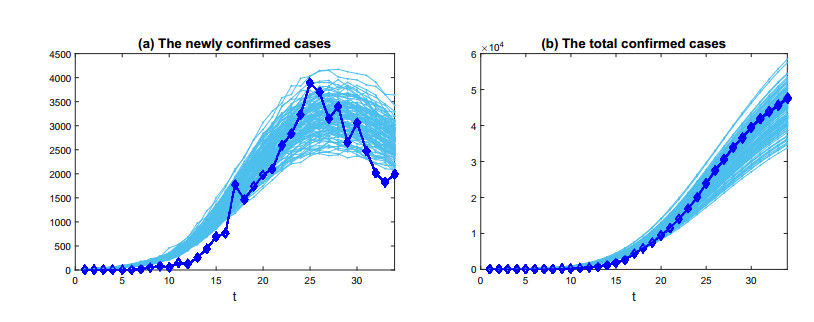
\includegraphics[scale=0.5]{img/page_de_garde.png} \\[1cm]
        \HRule \\[0.4cm]
        { \huge \bfseries LINMA2470 Stochastic Modelling \\[0.4cm] }
    
        \HRule \\[1.5cm]
        \textsc{\LARGE Simon Desmidt}\\[1cm]
        \vfill
        \vspace{2cm}
        {\large Academic year 2024-2025 - Q2}
        \vspace{0.4cm}
         
        
\includegraphics[width=0.15\textwidth]{img/epl.png}
        
        UCLouvain\\
    
    \end{center}
    \end{sffamily}
\end{titlepage}

\setcounter{tocdepth}{1}
\tableofcontents
\chapter{Reminders}
\section{General properties of probability}
\begin{itemize}
  \item $P[A\cup B]=P[A]+P[B]-P[1\cap B]$;
  \item $P[A|B] = \frac{P[A\cap B]}{P[B]} = \frac{P[AB]}{P[B]}$;
  \item $A$ and $B$ are independent iff $P[AB]=P[A]P[B]\Longrightarrow P[A|B]=P[A]$;
  \item $P[X\le x]=F_X(x)$ is the distribution function, i.e. a monotone increasing function of $x$ going from 0 to 1 when $x$ goes from $-\infty$ to $+\infty$.
  \item Its derivative is the density function $f_X(x)$ such that $f_X(x)\delta \approx P[x\le X\le x+\delta]$ for an infinitesimal $\delta$.
  \item A random variable $X$ is said to be memoryless if $\forall t,x>0$, $P[X>t+x|X>t]=P[X>x]$.
  \item Markov inequality (for a nonnegative random variable): $P[Y\ge y] \le \frac{\E[Y]}{y}$;
  \item Chebyshev inequality: $P[|Z-\E[Z]| \ge \varepsilon] \le \frac{\sigma_Z^2}{\varepsilon^2}$;
\end{itemize}
\section{Expectation and variance}
\begin{itemize}
  \item For a discrete random variable, $\E[X]= \sum_{n=-\infty}^\infty nP[X=n]$;
  \item For a continuous random variable, $\E[X]=\int_{-\infty}^\infty xf_X(x)dx$;
  \item $\E[X] = \int_0^\infty (1-F_X(x))dx$.
  \item $Var[X] = \sigma_X^2 = \E[(X-\E[X])^2] = \E[X^2] - \E[X]^2$;
\end{itemize}
\section{Law of large numbers}
Let $X_1,\dots,X_n$ be a series of independent and uniformly distributed (IID) random variables with expectation $\bar X$ and finite variance $\sigma_X^2$. Let $S_n = X_1+\dots +X_n$. Then, 
\begin{itemize}
  \item Weak version:
\end{itemize}
\begin{equation}
  \lim_{n\to \infty} P\left[|\frac{S_n}{n}-\bar X|\ge \varepsilon\right] = 0
\end{equation}
\begin{itemize}
  \item Strong version:
\end{itemize}
\begin{equation}
  \lim_{n\to \infty} P\left[\sup_{m\ge n}\left(\frac{S_m}{m}-\bar X\right)>\varepsilon\right] = 0\Longleftrightarrow \lim_{n\to \infty}\frac{S_n}{n}=X\qquad \text{with probability 1}
\end{equation}
\section{Central limit theorem}
\begin{equation}
  \lim_{n\to \infty} P\left[\frac{S_n-n\bar X}{\sqrt{n}\sigma}\le y\right] = \int_{-\infty}^y \frac{1}{\sqrt{2\pi}} e^{-\frac{x^2}{2}}dx
\end{equation}
\section{Exponential distribution}
\begin{itemize}
  \item $f_X(x)=\lambda e^{-\lambda x}$, for $x\ge 0$;
  \item $F_X(x)=1-e^{-\lambda x}$, for $x\ge 0$;
  \item $\E[X]=1/\lambda$.
  \item [$\rightarrow$] Note: the exponential distribution is memoryless.
\end{itemize}
\chapter{Poisson Processes}
A Poisson process $N(t)$ counts the number of arrivals with exponentially distributed inter-arrival times. 
\begin{equation}
  S_n = \sum_{i=1}^n X_i \qquad \qquad X_i \sim \exp(\lambda)
\end{equation}
$\forall n,t$, we have the relation $\{S_n\le t\}=\{N(t)\ge n\}$, where $S_n$ is a random variable telling at which time the $n$-th occurence appears.\\
\begin{itemize}
  \item [$\rightarrow$] Note: a Poisson process is memoryless: $P[Z_1>x]=e^{-\lambda x}$, with $Z_1$ be the duration of the time interval from $t$ until the first arrival after $t$.
\end{itemize}
For a Poisson process of rate $\lambda$, and any given $t>0$, the length of the interval from $t$ until the first arrival after $t$ is an exponentially distributed random variable. This random variable is idenpendent of both $N(t)$ and of the $N(t)$ arrival epochs before time $t$. It is also independent of $N(\tau)$, $\forall \tau \le t$.\\

Let us consider the process after $Z_1$, $Z_m$, the time until the $m$-th arrival after time $t$. It is independent of $N(t)$ and of the entier previous history of the process.\\
Let us denote $\tilde N(t,t') = N(t')-N(t)$. 
\begin{itemize}
  \item Stationary increments property: It has the same distribution as $N(t'-t)$, $\forall t'\ge t$ (stationary increments property);
  \item Independent increments property: For any sequence of times $0<t_1<\dots<t_k$, the set $\{N(t_1), \tilde N(t_1,t_2), \dots,\tilde N (t_{k-1}, t_k)\}$ is a set of independent random variables.
\end{itemize}
From the memoryless property, here is another definition of a Poisson process: \\
\begin{itemize}
  \item A Poisson process is a counting process that has the stationay and independent increment properties and such that 
\end{itemize}
\begin{equation}
  \begin{aligned}
    P[\tilde N(t, t+\delta)=0] &= 1-\lambda \delta +o(\delta)\\  P[\tilde N(t, t+\delta)=1] &= \lambda \delta +o(\delta)\\
    P[\tilde N(t, t+\delta)\ge2] &= o(\delta)
  \end{aligned}
\end{equation}
\section{\texorpdfstring{Distribution of $N(t)$}{Distribution of }}
$S_n$ is the sum $n$ IID random variables and $f_{S_n}$ is the convolution of $n$ times $f_X$:
\begin{equation}
  f_{S_n}(t) = \frac{\lambda^n t^{n}e^{-\lambda t}}{(n-1)!}
\end{equation}
From this, 
\begin{equation}\label{eq:poisson_distrib}
  P[N(t)=n-1] = \frac{(\lambda t)^{n}e^{-\lambda t}}{(n)!}
\end{equation}
and finally, 
\begin{equation}
  \E[N(t)] = \lambda t\qquad Var[N(t)] = \lambda t
\end{equation}
From equation \eqref{eq:poisson_distrib}, the Poisson process verifies the following probability conditions:
\begin{itemize}
  \item $P[\tilde N(t,t+\delta)=0]=1-\lambda \delta +o(\delta)$;
  \item $P[\tilde N(t,t+\delta)=1]=\lambda \delta +o(\delta)$;
  \item $P[\tilde N(t,t+\delta)\ge2]=o(\delta)$;
\end{itemize}
where we use a first-order approximation of the exponential term, with $o(\delta)$ its residual. As $o(\delta)$ is negligible, we can approximate the Poisson process as a Bernoulli process. 
\subsection{Combining Poisson processes}
Let $N_1(t)$ and $N_2(t)$ be tow independent Poisson processes. Let the process $N(t)=N_1(t)+N_2(t)$. We can show using the three properties above that $N(t)$ is a Poisson process with rate $\lambda_1+\lambda_2$.
\subsection{Subdividing a Poisson process}
Let $N(t)$ be a Poisson process with rate $\lambda$. We split the arrivals in 2 subprocesses $N_1(t)$ and $N_2(t)$. Each arrival of $N(t)$ is sent to $N_1(t)$ with probability $p$ and to $N_2(t)$ with probability $(1-p)$, each split being independent from all others. \\
Then, the resulting processes $N_1(t)$ and $N_2(t)$ are two independent Poisson processes with respective rate $p\lambda$ and $(1-p)\lambda$.
\subsection{Conditional arrival distribution}
The density probability function when we have $n$ Poisson processes, under the condition that $N(t)=n$, is
\begin{equation}
  f(s_1,\dots,s_n|N(t)=n)=\frac{n!}{t^n}
\end{equation}
From the previous results, we can compute that 
\begin{equation}
  P[S_1>\tau|N(t)=n]=\left(\frac{t-\tau}{t}\right)^n
\end{equation}
and the expectation is 
\begin{equation}
  E[S_1|N(t)=n] = \frac{t}{n+1}
\end{equation}
And from this, we derive that 
\begin{equation}
  P[X_i>\tau|N(t)=n] = \left(\frac{t-\tau}{t}\right)^n
\end{equation}
with expectation 
\begin{equation}
  E[X_i] = \frac{t}{n+1}
\end{equation}
And thus the density function is 
\begin{equation}
  f_{S_i}(x|N(t)=n) = \frac{x^{i-1}(t-x)^{n-i}n!}{t^n (n-i)!(i-1)!}
\end{equation}
\section{Non-homogenous Poisson processes}
A non-homogenous Poisson rocess $N(t)$ is a counting process with increments that are independent but not stationary, with
\begin{itemize}
  \item $P[\tilde N(t,t+\delta)=0]=1-\lambda (t)\delta + o(\delta)$;
  \item $P[\tilde N(t,t+\delta)=1]=\lambda (t)\delta + o(\delta)$;
  \item $P[\tilde N(t,t+\delta)\ge2]=o(\delta)$;
\end{itemize}
where $\tilde N(t,t+\delta)=N(t+\delta)-N(t)$. The time-varying arrival rate $\lambda(t)$ is assumed to be continuous and stricly positive.
\section{Bernoulli process approximation}
We can approximate the non-homogenous Poisson process with a Bernoulli process where the time is partitioned into increments of lengths inversely proportional to $\lambda (t)$ (i.e. using a nonlinear time scale).
\begin{itemize}
  \item $P[\tilde N(t,t+\epsilon/\lambda(t))=0]=1-\epsilon + o(\epsilon)$;
  \item $P[\tilde N(t,t+\epsilon/\lambda(t))=1]=\epsilon + o(\epsilon)$;
  \item $P[\tilde N(t,t+\epsilon/\lambda(t))\ge2]=o(\epsilon)$;
\end{itemize}
Letting $\epsilon$ tend to zero, we obtain
\begin{equation}
  P[N(t)=n]=\frac{(m(t))^ne^{-m(t)}}{n!}\qquad P[\tilde N(t,t')=n]=\frac{(m(t,t'))^n e^{-m(t,t')}}{n!}
\end{equation}
with 
\begin{equation}
  m(t)=\int_0^t \lambda(\tau)d\tau \qquad m(t,t')=\int_t^{t'} \lambda(\tau)d\tau 
\end{equation}
\section{Classification of queueing systems}
\begin{itemize}
  \item We note $A/B/k$ where $A$ is the type of distribution for the arrival process, $B$ for the service time and $k$ the number of servers.
\end{itemize}
We suppose that the arrivals wait in a single queue.
Commonly used letters are 
\begin{itemize}
  \item M: exponential distribution (for A) or Poisson process (for B);
  \item D: deterministic time intervals;
  \item E: Erlang distribution;
  \item G: general distribution.
\end{itemize}

\end{document}